\problemname{Vvvvvv}
Platform games is an old video game genre, where you move across platforms hanging in the air. Vvvvvv is a platform game where you cannot jump, but instead are able to switch between regular gravity, which causes you to fall downwards, and anti-gravity, which causes you to fall upwards. There are only three buttons in the game: the gravitational switch (G), the go-left-button (V) and the go-right-button (H).

Your task is to find a sequence of button presses which takes you through a maze-like level with platforms and walls, from a given start position to a given final position. In order to receive full points, the sequence needs to be as short as possible.

\begin{figure}[ht!]
\centering
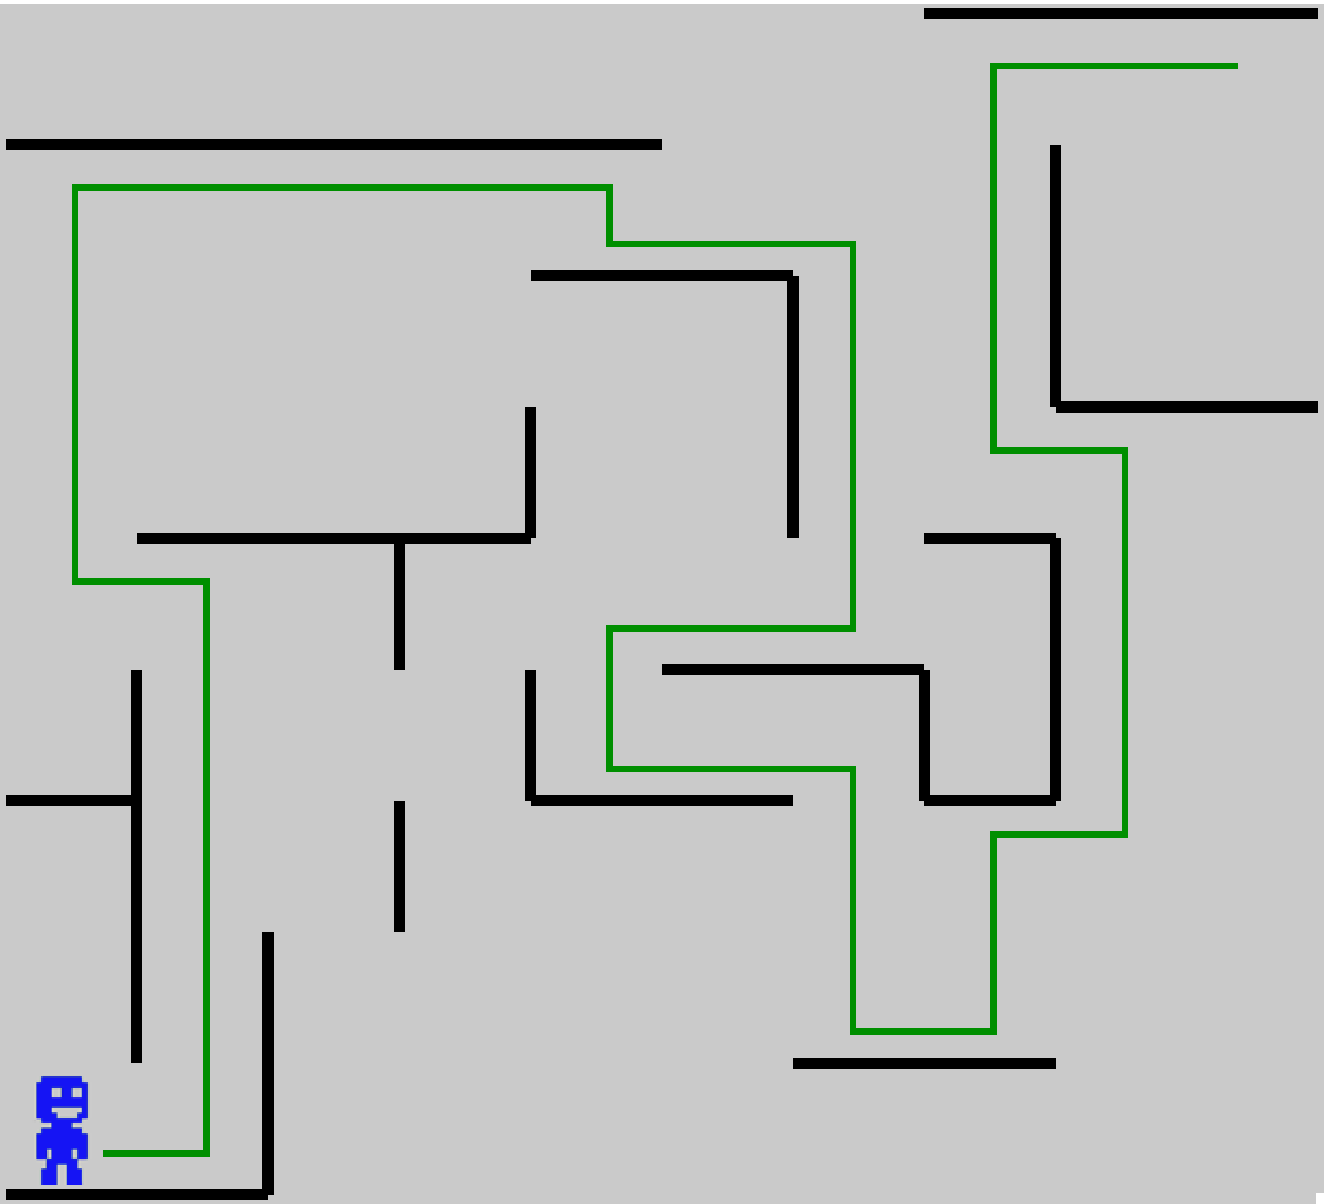
\includegraphics[width=0.6\textwidth]{spelplan.pdf}
\caption{The path given by the button presses given in the third sample.
\label{overflow}
\end{figure}

\section*{Input}
The first line of the input consists of three integers $W$, $H$, and $N$: the width of the level, the height of the level, and the number of line segments. Thereafter follows $N$ lines, each with four integers $x_1$, $y_1$, $x_2$, $y_2$, where $0 \le x_1, x_2 \le W$ and $0 \le y_1, y_2 \le H$. Each of these lines describe a line segments with end points $(x_1, y_1)$ and $(x_2, y_2)$. Every line segment is either horizontal or vertical, i.e. either $y_1=y_2$ or $x_1=x_2$ holds. The integer coordinate system can be said to divide the rectangular level into a grid, where the button V takes you one square to the left and H takes you one square to the right. If you are not standing on a platform after the movement you will fall (upwards or downwards) until you reach another platform. It is not possible to move to the left or right while falling. If you fall or walk out of the level, you lose the game. This also happens if you try to walk through a wall.

The start position is the lower left square, closest to the point (0, 0), with downwards gravity. The final position is the square in the upper right corner, closest to the point (W, H). There will always be a line segment under the start position and above the final position.

\section*{Output}
If there is a solution, the program should print a string containing a letter for each button press (chosen from G, V and H). The sequence should take you from the start position to the final position, and has to be shorter than $10000$ characters. You can arrive to the ending position with gravity in either direction, but you need to have stopped falling (see the third example below).

If there is no solution, the program should print the string \texttt{"Inte"} (without the quotation marks).

\section*{Scoring}
Your solution will be tested on a set of test case groups. In order to receive points for a group, you need to solve all test cases in the group.

\begin{tabular}{| l | l | p{5cm} | p{5cm} |}
	\hline
	Group & Points & Limits & Constraints \\ \hline
  1     & 20  & $W,H \le 10$, $N \le 25$, there is a solution with at most 10 moves & the sequence does not need to be as short as possible. \\ \hline
  2     & 15  & $W,H \le 20$, $N \le 200$, there is a solution where you do not need to use V & the sequence does not need to be as short as possible. \\ \hline
  3     & 15  & $W,H \le 50$, $N \le 2000$ & the sequence does not need to be as short as possible. \\ \hline
  4     & 20  & $W,H \le 10$, $N \le 50$ & the sequence needs to be as short as possible. \\ \hline
  5     & 30  & $W,H \le 100$, $N \le 5000$ & the sequence needs to be as short as possible. \\ \hline
\end{tabular}
